\newpage
\subsection{Textual; String Representation}
\texHeader
\hypertarget{stringRep tex}{}

\vspace{0.5cm}

\begin{itemize}
  
\item[$\blacktriangleright$] Closely following Fig.~\ref{fig:goal_stringRep}, create a nested \texttt{forEach} loop in \texttt{Box.toString}. The outer loop
pattern will be \texttt{[forAllPartitions]}, and the inner loop will be \texttt{[forAllCards]}. To call a method directly from a pattern's control flow,
surround the command with `\texttt{< >}' tags. Finally, before exiting the flow, return the newly-constructed \texttt{stringRep}.

\vspace{0.5cm}

\item[$\blacktriangleright$] Your eclass file should now resemble Fig.~\ref{fig:toStringFlow}

\vspace{0.5cm}

\begin{figure}[htp]
\begin{center}
  \includegraphics[width=0.6\textwidth]{eclipse_boxtoStringFlow}
  \caption{Control flow for \texttt{toString}}
  \label{fig:toStringFlow}
\end{center}
\end{figure}

\vspace{0.5cm}

\item[$\blacktriangleright$] Despite its complicated appearance, remember - the core idea behind this method is to create a path to every item in
\texttt{Box}. Then from the control flow (which we've already established), call a helper function to complete the action. This means both patterns need only
create their two relevant object variables each, then link them together.

\item[$\blacktriangleright$] Confirm your patterns match Fig.~\ref{fig:toStringPatterns} before continuing.

\begin{figure}[htp]
\begin{center}
  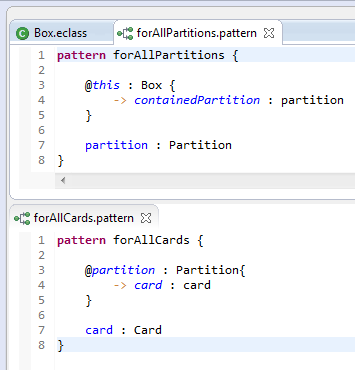
\includegraphics[width=0.6\textwidth]{eclipse_toStringPatterns}
  \caption{ForEach patterns needed for \texttt{toString}}
  \label{fig:toStringPatterns}
\end{center}
\end{figure}

\vspace{0.5cm}

\item[$\blacktriangleright$] As crazy at it may seem, that's it!  To
see how this SDM is represented visually, check out Fig.~\ref{fig:sdm_tostring_5}.

\end{itemize}
